%%
%% This is file `sample-acmlarge.tex',
%% generated with the docstrip utility.
%%
%% The original source files were:
%%
%% samples.dtx  (with options: `acmlarge')
%% 
%% IMPORTANT NOTICE:
%% 
%% For the copyright see the source file.
%% 
%% Any modified versions of this file must be renamed
%% with new filenames distinct from sample-acmlarge.tex.
%% 
%% For distribution of the original source see the terms
%% for copying and modification in the file samples.dtx.
%% 
%% This generated file may be distributed as long as the
%% original source files, as listed above, are part of the
%% same distribution. (The sources need not necessarily be
%% in the same archive or directory.)
%%
%%
%% Commands for TeXCount
%TC:macro \cite [option:text,text]
%TC:macro \citep [option:text,text]
%TC:macro \citet [option:text,text]
%TC:envir table 0 1
%TC:envir table* 0 1
%TC:envir tabular [ignore] word
%TC:envir displaymath 0 word
%TC:envir math 0 word
%TC:envir comment 0 0
%%
%%
%% The first command in your LaTeX source must be the \documentclass command.
\documentclass[acmlarge]{acmart}

\usepackage{color}
\usepackage{listings}
\lstset{language=Go,
  basicstyle=\ttfamily\scriptsize,
  keywordstyle=\color{blue}\ttfamily,
  stringstyle=\color{red}\ttfamily,
  commentstyle=\color{green}\ttfamily}
%%
%% \BibTeX command to typeset BibTeX logo in the docs
\AtBeginDocument{%
  \providecommand\BibTeX{{%
    \normalfont B\kern-0.5em{\scshape i\kern-0.25em b}\kern-0.8em\TeX}}}

%% Rights management information.  This information is sent to you
%% when you complete the rights form.  These commands have SAMPLE
%% values in them; it is your responsibility as an author to replace
%% the commands and values with those provided to you when you
%% complete the rights form.
\setcopyright{acmcopyright}
\copyrightyear{2022}
\acmYear{2022}
\acmDOI{}


%%
%% These commands are for a JOURNAL article.
\acmJournal{POMACS}
\acmVolume{37}
\acmNumber{4}
\acmArticle{1}
\acmMonth{8}

%%
%% Submission ID.
%% Use this when submitting an article to a sponsored event. You'll
%% receive a unique submission ID from the organizers
%% of the event, and this ID should be used as the parameter to this command.
%%\acmSubmissionID{123-A56-BU3}

%%
%% The majority of ACM publications use numbered citations and
%% references.  The command \citestyle{authoryear} switches to the
%% "author year" style.
%%
%% If you are preparing content for an event
%% sponsored by ACM SIGGRAPH, you must use the "author year" style of
%% citations and references.
%% Uncommenting
%% the next command will enable that style.
%%\citestyle{acmauthoryear}

%%
%% end of the preamble, start of the body of the document source.
\begin{document}

%%
%% The "title" command has an optional parameter,
%% allowing the author to define a "short title" to be used in page headers.
\title{Paper Reading of \textit{Time, Clocks, and the Ordering of Events in a Distributed System}}

%%
%% The "author" command and its associated commands are used to define
%% the authors and their affiliations.
%% Of note is the shared affiliation of the first two authors, and the
%% "authornote" and "authornotemark" commands
%% used to denote shared contribution to the research.
\author{Yiwei Yang}
\email{yangyw@shanghaitech.edu.cn}
\orcid{0000-0001-8011-5868}
\affiliation{
  \institution{ShanghaiTech University}
  \streetaddress{1 R.D. Zhongke}
  \city{Shanghai}
  \state{Shanghai}
  \country{China}
  \postcode{21210}
}

%%
%% By default, the full list of authors will be used in the page
%% headers. Often, this list is too long, and will overlap
%% other information printed in the page headers. This command allows
%% the author to define a more concise list
%% of authors' names for this purpose.
\renewcommand{\shortauthors}{Trovato and Tobin, et al.}

%%
%% The abstract is a short summary of the work to be presented in the
%% article.
\begin{abstract}
  The paper presents a fundemantal concept for the ordering of an event in a distributed system.
  And once we have the formal definition of ordering, how we can use it to solve synchronization
  problems. Happens before, or partial ordering of events without precise physical time in the system
  is the assurance of Lamport Clock to be defined. In distributed mutual exclution, the must release
  granted resource before can be granted again, thhey should grant resources in order they are made, and
  every rquest should be eventually granted, assuming the process will not fail. A naive implementation of
  Lamport Clock is vector clock to store all nodes' time as vector. Eventually, it formally defined physical clocks
  with distributed implementation. Based on that, the example of Network Time Protocol is introduced.
\end{abstract}

%%  
%% The code below is generated by the tool at http://dl.acm.org/ccs.cfm.
%% Please copy and paste the code instead of the example below.
%%
\begin{CCSXML}
  <ccs2012>
  <concept>
  <concept_id>10010520.10010553.10010562</concept_id>
  <concept_desc>Distributed System~Lamport Clocks</concept_desc>
  <concept_significance>500</concept_significance>
  </concept>
  <concept>
  <concept_id>10010520.10010575.10010755</concept_id>
  <concept_desc>Vector Clocks~Physical Clocks</concept_desc>
  <concept_significance>300</concept_significance>
  </concept>
  </ccs2012>
\end{CCSXML}

\ccsdesc[500]{Computer systems organization~Embedded systems}
\ccsdesc[300]{Computer systems organization~Redundancy}
\ccsdesc{Computer systems organization~Robotics}
\ccsdesc[100]{Networks~Network reliability}

%%
%% Keywords. The author(s) should pick words that accurately describe
%% the work being presented. Separate the keywords with commas.
\keywords{distributed system, lamport clock, sequantial consistency, NTP}


%%
%% This command processes the author and affiliation and title
%% information and builds the first part of the formatted document.
\maketitle

\section{Strong Point of the paper}


\subsection {\texttt{Ordering}}
The author specify the sequentrial consistency(every core sees same read/write order), and Release consistency(every core sees write in unlock order)
Happened before, which is the partial consistency, means the smalles relation satisfying:
\begin{itemize}
  \item Either one event on the same process is ordered.
  \item Messege ordered after associated message sends.
  \item As shown in the left graph down below, we can conclude the
        transitivity that $a \rightarrow b$ and $b \rightarrow c$ implies $a \rightarrow c$
\end{itemize}

We can write the state in go using structs and message is to maintain the process id and the type whether is Ack or Processing,
and time is the logical time:

\begin{lstlisting}

  type LamportLockState struct {                  type Message struct {
    time int                                      	Type int // Message type
    proc int                                      	Proc int // Origin process
    seen     []int                                	Time int // Logical time on origin
    channels []chan Message                       }
    reqs     *MessageHeap                         
    lock sync.Mutex                               type MessageHeap []Message
  }                 
  \end{lstlisting}


\begin{figure}[h]
  \centering
  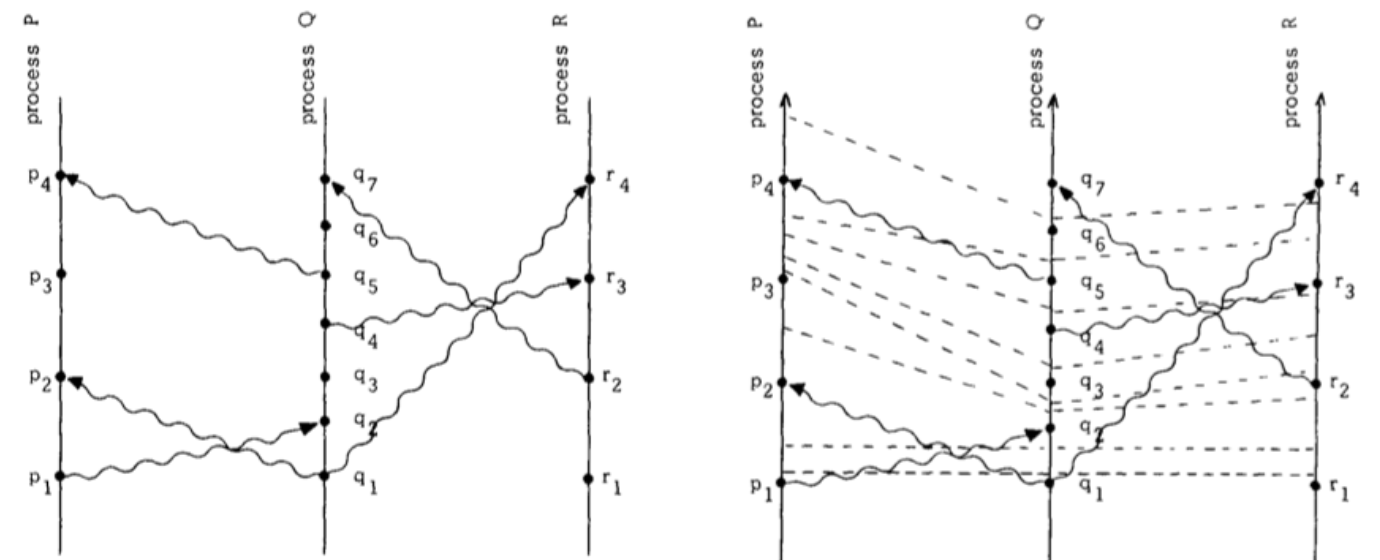
\includegraphics[width=\linewidth]{partial_order.png}
  \caption{Partial ordering of events in the system. Vertical bars are processes.
    Wavy arrows are messages. A dot is an event. Time elapses bottom up.}
\end{figure}

The definiation of happened before actually break the convention that the
system must have physical clocks every node for keeping precise physical
time which may have clock skewing problems.

\subsection{Logical(Lamport) Clocks}
The logical clocks can be simply defined by clock condition:
\begin{itemize}
  \item if $a \rightarrow b$ then Clock $(a)<\operatorname{Clock}(b)$.
  \item If $a$ is the sending of a message by process $P_{i}$ and $b$ is the receipt
        of that message by process $P_{j}$ then Clo ${ }_{i}(a)<\operatorname{Clock}_{j}(b)$
\end{itemize}
By the dotted line, the condition assures the transmission of timestamp data should appear and across between concrete lines. One possible
implementation using this timestamp is:

\begin{itemize}
  \item \textbf{C1} Each process $P_{i}$ increments $C_{i}$ between any two successive events
  \item \textbf{C2} \begin{itemize}
          \item Send $T_{m}=C_{i}(a)$ along with the message from $a$.
          \item Upon receiving that message, $P_{j}$ sets its $C_{j}$ to be $\geq$ its present value and $>T_{m}$
        \end{itemize}
\end{itemize}

In Go implementation:

\begin{lstlisting}
func (state *LamportLockState) processMessage(m Message) {        } else if m.Type == MessageRelease {       
  // update the process-time vector and current time <- C2          // release previous request       
  state.seen[m.Proc] = m.Time                                       kept := make([]Message, 0)               
  if m.Time > state.time {                                          for state.reqs.Len() > 0 {             
    state.time = m.Time                                              req := heap.Pop(state.reqs).(Message)         
  }                                                                   if req.Proc != m.Proc {                           
                                                                      kept = append(kept, req) 
  // if needed (i.e. not just a MessageAck), update request heap      }       }      
  if m.Type == MessageRequest {                                     for _, req := range kept 
    // new request: add to queue                                     {                      
    heap.Push(state.reqs, m)                                          heap.Push(state.reqs, req)                   
    // reply with an acknowledgement <- C1                          }                                     
    state.sendAckMsg(m.Proc)                                      }
                                                                 }      
  \end{lstlisting}

\subsection{Vector Clocks}
\begin{figure}[h]
  \centering
  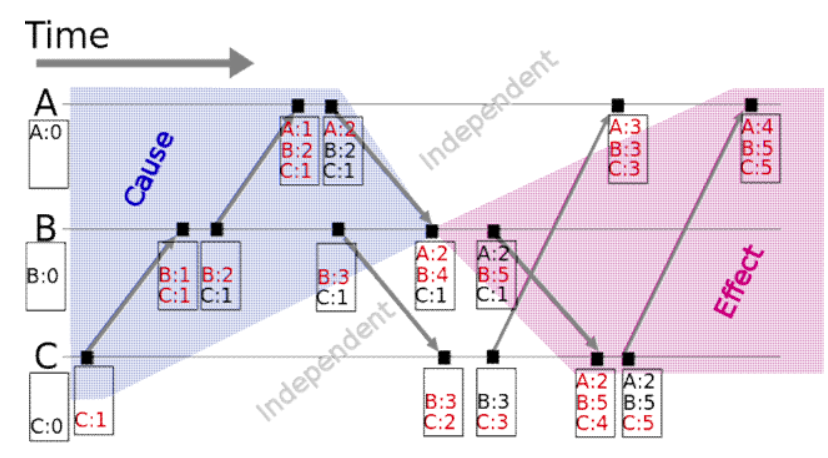
\includegraphics[width=\linewidth]{vec_lock.png}
  \caption{$\mathbf{V}<\mathbf{V}^{\prime}$ if $\leq$ on each element and $<$ on at least one element}
\end{figure}
We have problem that the system will halt if one process fails. Ti Generize, 
\subsection{Physical Clocks}

\subsection{Network Time Protocol}



\section{Weak Point of the paper}
\subsection {No strongly software implementable module for programming} To ensure the parcial order, we have
\subsection{Many concepts are not fully documented at that time} Produces colored hyperlinks.


\section{Possible Refinement to the idea}

\subsection {Better implementation for fault tolerance}
Undo Logging
Snapshotting
2PL/MVCC
% Go 四叉树
\subsection{Better implementation for NTP protocol} Produces colored hyperlinks.\cite{HFT-PTP-NTP} %beter NTP portocol



\bibliographystyle{ACM-Reference-Format}
\bibliography{clocks_and_the_ordering_of_events_in_a_distributed_system}

\end{document}
\endinput
%%
%% End of file `sample-acmlarge.tex'.
